% ============================================================================
%  Beautified Is Not Forged -- paper v10 (2026-10-28): main_v9.tex with the 34 wording-only edits of
%  HUMANIZER_AUDIT_V9_20261028.md applied by make_v10_humanize.py (repeated clauses varied, punch sentences folded in,
%  the thirteen longest sentences split, two coined phrases and two "therefore" removed). No number, interval, citation,
%  cross-reference or source comment changed; no claim strengthened or weakened. Supplement: supplement_v10.tex.
%  Former header of v9 (2026-10-28): main_v8.tex with CONSISTENCY_AUDIT_20261023 items M01-M25 applied,
%  Addenda 48 (both seeds), 49, 54 (GPUPixel), 57 (face vs context), 61 (context matching) and 62 (identity on Celeb-DF-B)
%  written in, the prevalence \todo removed (no prevalence is claimed). Changes are listed in V9_CHANGES.md.
%  Former header of v8 (2026-10-22). Restructured as an analysis / evaluation paper
%  (arXiv + IJCB 2027, IEEE two-column, 8 pages excluding references) following
%  docs/RESEARCH_CRITIQUE_20261021b.md (Sec. 9-10) and the benchmark-paper template (five pillars, six-part
%  introduction, bold Finding sentences). Headline numbers come from docs/capstone/MAIN_CLAIMS_20261022.md,
%  which is generated from results/research/alipair_zeroshot_20260929/main_claim_A.py and
%  results/research/celebdfb_v2_20260927/fair_cdfb.py. Every number in the text carries a % comment naming the
%  result file it was read from. Changes against main_v7.tex, what moved to the supplement, and the numbers that
%  could not be sourced (left as \todo{}) are listed in V8_CHANGES.md. main_v7.tex is untouched.
%
%  BIBLIOGRAPHY: refs_v8.bib (= refs_v6.bib + mirabet2025, ict2022, idreveal2021, yin2026). Supplement: supplement_v8.tex.
%  2026-10-22 (cut to 8 body pages): Table "prior evaluations" moved to the supplement (S-tab:compare); identity subsection
%  to one paragraph; Related Work halved; placeholder box replaced by figs/fig_twoaxis_v8 (make_fig_twoaxis_v8.py).
%
%  2026-10-22 (method figure): figs/fig_method_v8b (figs_tikz/fig_method_v8b.tex + make_fig_method_v8b.py) at the start of
%  Sec. I, "System and training recipe" paragraph in Sec. IV; fig_bandenergy_v8b and fig_sic_curve_v8b moved to the supplement.
%  TABLES reused from tables/: tab_sic.tex (Addendum 46 family, READOUT46.md). All other tables are written inline
%  below with per-cell source comments. FIGURES (2026-10-22 redesign, FIGURES_V8B.md): figs/fig_teaser_v8b, fig_exposure_v8b,
%  fig_bandenergy_v8b, fig_sic_curve_v8b, fig_twoaxis_v8b, each from make_fig_<name>_v8b.py reading the result files.
% ============================================================================
\documentclass[conference]{IEEEtran}
\IEEEoverridecommandlockouts
\usepackage[T1]{fontenc}\usepackage{newtxtext}   % Times clone that compiles with pdfLaTeX (IEEE PDF eXpress, arXiv) and with tectonic
\usepackage{cite}
\usepackage{amsmath,amssymb,amsfonts}
\usepackage{graphicx}
\usepackage{booktabs}
\usepackage{array}
\usepackage{adjustbox}
\usepackage{xcolor}
\usepackage{url}
\usepackage{capt-of}
\usepackage{xr-hyper}
\usepackage[hidelinks]{hyperref}
\newcommand{\ours}{\textsc{Ours}}
\newcommand{\oursB}{\textsc{Ours}, forgery head only}   % not used in the body; needed because xr-hyper reads supplement captions that use them
\newcommand{\oursF}{\textsc{Ours}, full model}
\externaldocument[S-]{supplement_v10}
\graphicspath{{figs/}}
\renewcommand{\dbltopfraction}{0.95}
\renewcommand{\topfraction}{0.95}
\renewcommand{\textfraction}{0.05}
\raggedbottom

\begin{document}

\title{Beautified Is Not Forged: A Two-Direction Measurement of Face-Forgery Detectors under Skin Smoothing}

\author{\IEEEauthorblockN{Anonymous submission}}

\IEEEaftertitletext{\vspace{-0.6\baselineskip}\begin{center}
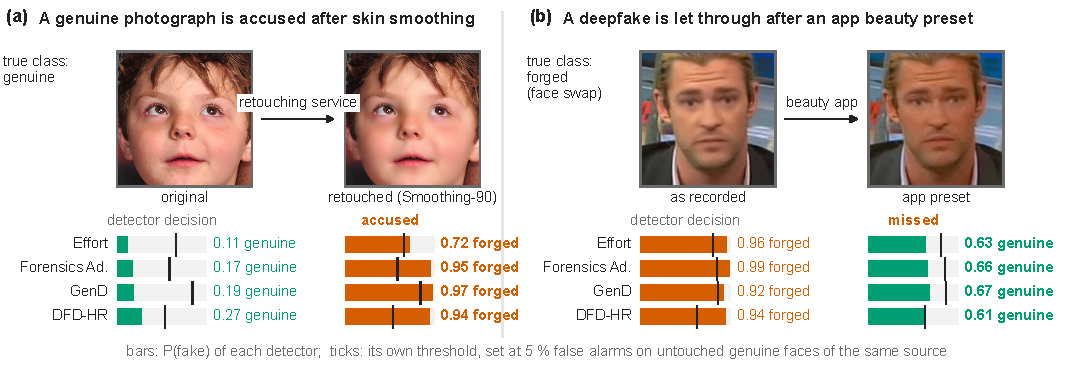
\includegraphics[width=0.98\textwidth]{fig_teaser_v9}
\captionof{figure}{One cue, two errors. (a) A genuine FFHQ photograph and its render by a commercial retouching service
(skin smoothing, strongest level): the four CLIP-based detectors call the original genuine and the retouched copy forged.
(b) A Celeb-DF-B face-swap video as recorded and after an app beauty preset: the same detectors catch the deepfake as
recorded and miss it after the preset. Bars are $P(\text{fake})$, ticks are each detector's own threshold, set where it
accuses 5\% of the untouched genuine faces of the same source; (b) uses the video mean over 32 frames. Across seventeen
published detectors the pattern is the rule, not the exception (Fig.~\ref{fig:dirs}).}
% figs/fig_teaser_v9.pdf, make_fig_teaser_v9.py: (a) published_scores_<det>.npz stem 17003, orig_0 / Smoothing_90, threshold =
% 95th pct of orig_0 (Effort 0.11 -> 0.72, thr 0.66; Forensics Adapter 0.17 -> 0.95, thr 0.59; GenD 0.19 -> 0.97, thr 0.84;
% DFD-HR 0.27 -> 0.94, thr 0.54). (b) celebdfb_v2_20260927/scores_v3/<det>.npz video id17_id35_0000, means over frames,
% threshold = 95th pct of real/ (Effort 0.96 -> 0.63, thr 0.81; FA 0.99 -> 0.66, thr 0.85; GenD 0.92 -> 0.67, thr 0.86;
% DFD-HR 0.94 -> 0.61, thr 0.63); frame f05 shown (its own scores: Effort 0.97 -> 0.44, FA 1.00 -> 0.67, GenD 0.89 -> 0.70,
% DFD-HR 0.99 -> 0.74).
\label{fig:teaser}
\end{center}\vspace{0.1\baselineskip}}

\maketitle

\begin{abstract}
Published face-forgery detectors read skin smoothing as forgery evidence, and the error runs in both directions: a genuine
face smoothed by a retouching service is accused, and a deepfake beautified by an app preset is let through. We score seventeen published detectors on pixel-aligned retouching pairs and on app-beautified deepfake videos with one decision rule. Fifteen of the seventeen score the smoothed genuine face above its own original
in 89--99\% of pairs,
% docs/capstone/MAIN_CLAIMS_20261022.md, Direction A table (main_claim_A.json)
and fourteen miss 3--22 points more of the beautified deepfakes than of the untreated ones once re-encoding is controlled for.
% results/research/celebdfb_v2_20260927/FAIR_cdfb.md, "rise from beautification alone" column, detectors with CI above 0
Controlled training arms show that the class that receives smoothed views during training
sets the sign of the error, and that exposure to smoothing is necessary and sufficient for it. The cue is a face smoother than
its own context, not blur and not the boundary line. Four repairs, from a conditional threshold to a consistency loss, each reduce to moving the operating point, because under smoothing the scores of genuine and forged faces coincide. The one channel we tested that beautification leaves intact is identity against a reference of the claimed person: on app-beautified face swaps it misses 0.6\% of the forgeries at the false-alarm rate where texture
detectors miss 46--72\%,
% results/research/retouch_unified_20260929/CDFB_ID.md (Addendum 62), last column
but its threshold still has to know about beautification. Manifests, scorer, paired reader, result files and the pre-registration log are released.
\end{abstract}

% ----------------------------------------------------------------------------
\section{Introduction}
\label{sec:intro}
\begin{figure*}[t]
\centering
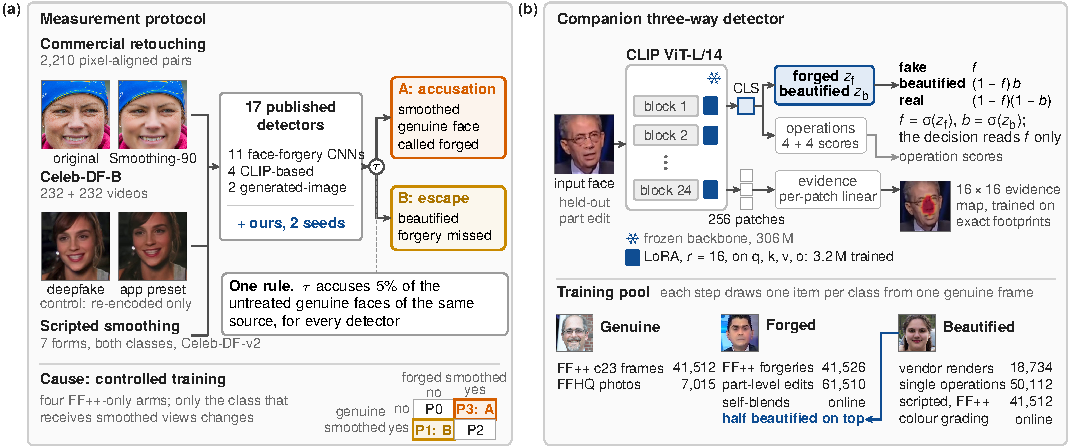
\includegraphics[width=\textwidth]{fig_method_v10}
\caption{Overview. (a) The measurement: beautified genuine and forged faces from three sources are scored by seventeen
published detectors and ours, each thresholded at the score $\tau$ that accuses 5\% of the untreated genuine faces of the same
source; Direction A counts smoothed genuine faces called forged, Direction B beautified forgeries missed. The cause is tested
with four training arms that differ only in which class receives smoothed views (Sec.~\ref{sec:exposure}). (b) The companion
detector of Sec.~\ref{sec:companion}: a frozen CLIP ViT-L/14 with rank-16 LoRA, a forged and a beautified logit on the CLS token
(the decision reads only $f$), auxiliary operation scores and a $16\times16$ evidence map on the patch tokens (shown on a
held-out part-level forgery). Each training step builds one genuine, one forged and one beautified item from the same genuine
frame; half of the forged items are beautified as well, so both classes see beautification.}
% figs/fig_method_v8b.pdf: figs_tikz/fig_method_v8b.tex, thumbnails and evidence map by make_fig_method_v8b.py (main model
% clipe5_s20260929); counts and recipe checked against results/research/retouch_unified_20260929/manifest_train.tsv,
% train_ru_clipe5_s20260929.log and train_ru5.py (FIGURES_V8B.md, Fig. 0).
\label{fig:method}
\end{figure*}
A person takes a selfie, lets a beauty app or a retouching service smooth the skin, and uploads it. The face is the same person with the same
expression at the same moment; only the skin texture has changed. If that photograph reaches a forgery detector during
content moderation, a remote identity check or fact-checking, it should be called genuine. If a deepfake of the same person
passes through the same app, it should still be called forged. Beautification edits the pixels a detector inspects but
changes neither who is shown nor what the person does. Skin smoothing, whitening, eye enlarging and face slimming are offered
by camera apps, AR filters and retouching services~\cite{openfilter2022,retouchingffhq,libourel2024}; we make no claim about
how often they are used. Fig.~\ref{fig:teaser} shows what happens today on one photograph and one video; across the seventeen published detectors we
scored, the retouched copy outranks the original in 89--99\% of pairs for fifteen of them (Fig.~\ref{fig:dirs}).

Three evaluations have looked at this. Libourel et al.~\cite{libourel2024} released Celeb-DF-B and report video-level AUC
drops for three detectors under four app presets, without separating the two classes of error. Saeed et al.~\cite{saeed2025}
apply six enhancement filters to deepfakes and measure how many escape six detectors; genuine faces are never enhanced, so
the accusation direction is not measured. Concas et al.~\cite{concas2025} apply one smoothing filter to genuine and forged
test images of two CNNs they trained (AlexNet, VGG19) and observe that the two move in opposite directions, which they attribute to the detector (``the underlying system'') without tracing it to training. Each study measures one direction with a handful of detectors, and none tests a cause. In generated-image detection, Ricker et
al.~\cite{ricker2026biasid} showed that training with JPEG on one class only flips the sign of the error, with two of the
four exposure cells. The implicit assumption shared by robustness benchmarks~\cite{deeperforensics2020,moire2025,hendrycks2019}
is that a benign edit degrades a detector symmetrically, so that AUC under the edit is the number to report. We show that for
skin smoothing the degradation has a sign, that the sign is set in training, and that AUC hides it.

We ask three questions. RQ1: across the detector families in use today, how often is a smoothed genuine face accused and
how often does a smoothed forgery escape, under one rule? RQ2: where does the cue come from, which part of the edit carries
it, and does it depend on what the detector was trained on? RQ3: can a decision rule or a training rule remove it without
giving up detection of untreated forgeries?

Answering them needs four things. Both directions must be read on the same detector with the same rule; pairs must be read without a threshold where the original exists; re-encoding must be controlled and the cause tested by intervention on training; and uncertainty must be reported at the sampled unit, pairs or videos rather than frames.

We build such a measurement from three beautification sources in the main text: commercial retouching pairs, app-beautified
deepfake videos and scripted smoothing (colour-filter and AR sources are in the supplement). We replicate the accusation on an
open-source beauty engine and score seventeen published detectors and a family of our own controlled arms with one rule (Fig.~\ref{fig:method}). Our contributions are:
\begin{itemize}
\item A two-direction evaluation protocol and its results on seventeen detectors (Sec.~\ref{sec:protocol},
Findings~1--2): on pixel-aligned commercial retouching pairs fifteen detectors rank the retouched copy above its original
in nearly every pair, and on app-beautified deepfake videos fourteen miss more forgeries once re-encoding is removed; the
skin smoothing operation by itself produces the shift.
\item The cause by intervention (Findings~3--4). A complete $2\times2$ training-exposure design on face forgery, extending Ricker et al.~\cite{ricker2026biasid} to all four cells, shows that the class receiving smoothed views sets the
sign of the error, that removing smoothing from the views brings the error back and that smoothing alone sets it. A
band-energy analysis and an edge-treatment ablation then show that the cue is the contrast between a flattened face and its
untouched surroundings, neither texture loss nor the boundary line.
\item Negative results that bound what a fix can do (Findings~5--6): no threshold rule separates smoothed genuine from
smoothed forged faces for any of the detectors, and four repairs (a conditional threshold, a routed expert, a consistency
loss, test-time context matching) each turn out to move the operating point rather than restore separation, since every
model loses separability when both classes are smoothed.
\item The channel that survives (Finding~7): identity against a reference of the claimed person keeps its separation under
real app presets but not its operating point; the channel is prior art and we claim no fusion with it.
\item An audit reference (Sec.~\ref{sec:companion}): a three-way detector that sees smoothing on both classes, with a
forgery-head-only control on the same data that does as well; it is trained on more data than the published detectors and
is not ranked against them.
\end{itemize}

% ----------------------------------------------------------------------------
\section{Measurement Protocol}
\label{sec:protocol}
\textbf{Classes.} A face is \emph{forged} if it shows a person, an expression, a motion or speech that was not captured:
another identity in whole or in part, a reenactment, or a facial feature replaced by new content. It is \emph{beautified} if
its colour, tone, skin texture or the shape of the person's own features were edited after capture while identity,
expression and pose stay those of the capture. The label follows what changed, not the tool, and a beautified forgery is
forged. Cases near the boundary are listed in the supplement (Table~\ref{S-tab:labels}); the boundary is stated, not
measured.

\textbf{One rule, both directions.} Every detector is scored by its own $P(\text{fake})$ with the threshold that accuses
5\% of each source's untreated genuine faces. Under beautification we report the false-alarm rate FA on beautified genuine
faces (Direction A, the accusation) and the miss rate MISS on beautified forgeries (Direction B, the escape); a forgery that a
three-way model sends to its beautified class counts as a miss. Where the untouched original of each beautified face exists
we also report the share of pairs in which the beautified face scores above its own original, which needs no threshold and
is the quantity of Fig.~\ref{fig:dirs}. Intervals are 95\% percentile bootstraps over pairs or videos with the threshold
re-estimated in every draw (1,000 draws), and differences between models use identical draws; a second bootstrap with
identities as the unit changes none of the headline intervals (Table~\ref{S-tab:identity}).

\textbf{Sources.} \emph{Commercial retouching}: 2,210 FFHQ photographs~\cite{ffhq} and their renders by one retouching
service from RetouchingFFHQ~\cite{retouchingffhq}, pixel-aligned, four operations at three levels; the strongest skin
smoothing (Smoothing-90) is the headline condition, and the other operations serve as controls that pass through the same
service and encoder. No model was trained on this service, but our companion model saw renders of the two other services of the same release (Sec.~\ref{sec:companion}), and the service was read during the study, so it is an analysis set rather than a blind test.

\emph{App-beautified deepfake videos}: Celeb-DF-B~\cite{libourel2024}, 232 genuine and 232 forged
Celeb-DF-v2 videos per condition (as recorded, re-encoded, beautified by one of four Instagram presets), 32 frames each; the
rise in misses under a preset is read minus the rise under re-encoding, so what remains is the beautification alone.

\emph{Scripted smoothing}: 4,016 Celeb-DF-v2 test frames (1,348 genuine, 513 videos)
% results/research/retouch_unified_20260929/FINDINGS.md, Addendum 38 header
under seven forms applied to both classes: a whole-crop bilateral filter at three strengths, a $5\times5$ median, a 50\%
Gaussian blend, and a bilateral filter confined to the landmark face hull at two strengths (\emph{face-local}, background
untouched). \emph{Calibration renders}: FF++ validation genuine frames under the same forms, used only to fit the threshold
rule of Finding~5. \emph{Untreated detection}: Celeb-DF-v2~\cite{celebdf}, DFD~\cite{dfd} and DF40~\cite{df40}. Counts,
crops and preprocessing are in the supplement.

\textbf{What is not a clean source.} Instagram AR filters rendered through OpenFilter~\cite{openfilter2022} (FairBeauty, B-LFW) were scored but are excluded as evidence, for one reason: the filter cannot be separated from the capture pipeline. The AR engine re-renders the face through its own capture path, and there
is no no-filter pass through that path. A model trained on such pairs still calls 94.8\% of filtered images beautified when the face is greyed out,
% supplement_v7.tex Sec. S-excluded (AR beauty filters paragraph)
and a multi-operation arm whose AR accusation did not fall calls only 18.2\% of the FairFace originals genuine (Sec.~\ref{S-sec:ar}).
% FINDINGS.md 2026-10-22 16:40, Addendum 56 pipeline control (ar_pipeline_control, 599 pairs)
Every detector, ours included, accuses 10--97\% of these renders (Table~\ref{S-tab:ar}); we report that as a limitation and
make no claim on AR filters.
% tables/tab_v6b_ar.tex: FairBeauty 10.7 (SPSL) .. 85.9 (DFD-HR); B-LFW 12.0 .. 96.6 (GenD); NPR B-LFW 0.0 saturated

\textbf{Detectors.} Eleven face-forgery CNNs (Xception~\cite{xception}, EfficientNet-B4~\cite{efficientnet},
F3Net~\cite{f3net}, SPSL~\cite{spsl}, UCF~\cite{ucf}, RECCE~\cite{recce}, CORE~\cite{core}, SRM~\cite{srm}, SBI~\cite{sbi},
CADDM~\cite{caddm}, LAA-Net~\cite{laanet}), four CLIP ViT-L/14 detectors (Effort~\cite{effort}, Forensics
Adapter~\cite{forensicsadapter}, GenD~\cite{gend2026}, DFD-HR~\cite{dfdhr2026}) and two generated-image detectors
(UnivFD~\cite{univfd}, NPR~\cite{npr}), all with released weights, each on its own crop. Table~\ref{S-tab:reproduce} sets the released checkpoints against their published Celeb-DF-v2 numbers: the eight DeepfakeBench CNNs land within 0.035 frame AUC of the published value, Forensics Adapter and GenD reproduce their video AUC, and Effort and DFD-HR fall 0.02--0.03 short and are used as released (Sec.~\ref{sec:limits}). CADDM and LAA-Net reproduce their video AUC within 0.011 on their own crops (Sec.~\ref{S-sec:baselines}); SBI, UnivFD and NPR have no comparable published number on this protocol. NPR saturates at 1.0 on the
retouching source and is reported as such. Table~\ref{S-tab:compare} compares this protocol with the prior evaluations of Sec.~\ref{sec:intro} feature by feature.


% ----------------------------------------------------------------------------
\section{Findings}
\label{sec:findings}

\subsection{Direction A: the accusation}
\label{sec:accuse}
\begin{table}[t]
\centering
\caption{Direction A on 2,210 pixel-aligned retouching pairs. Above own: share of pairs in which the Smoothing-90 render
scores above its own original (50 means no shift). FA: share of renders above the threshold that accuses 5\% of the
originals. Right: the same FA for whitening, face slimming and eye enlarging at their strongest level. Brackets: 95\%
bootstrap over pairs. NPR scores everything at 1.0; --: not scored. Bold: above own closest to 50 and the lowest Smoothing-90 FA (NPR not ranked). Ours (bold): the three-way detector of Sec.~\ref{sec:companion}, two seeds; it was trained on renders of two other services from the same RetouchingFFHQ release and on more data than the published detectors, so its rows are a reference, not a ranking.}
\label{tab:dirA}
\scriptsize
\setlength{\tabcolsep}{2.3pt}
\begin{tabular}{@{}l cc ccc@{}}
\toprule
 & \multicolumn{2}{c}{Smoothing-90} & \multicolumn{3}{c}{FA, other operations (level 90)} \\
\cmidrule(lr){2-3}\cmidrule(lr){4-6}
Detector & above own [CI] & FA [CI] & white & slim & eye \\
\midrule
% Columns 2-3: results/research/alipair_zeroshot_20260929/MAIN_CLAIM_A.md (main_claim_A.json).
% Columns 4-6: docs/paper_v2/tables/tab_v6b_perop.tex (make_tables_v6b.py from published_ali.json).
Xception & 95.2 [94.3, 96.1] & 51.6 [49.5, 53.7] & 5.7 & 3.7 & 4.6 \\
EfficientNet-B4 & 93.7 [92.6, 94.7] & 36.3 [34.3, 38.4] & 5.1 & 4.0 & 4.7 \\
F3Net & 97.8 [97.1, 98.3] & 50.6 [48.5, 52.6] & 5.4 & 4.2 & 4.4 \\
SPSL & 97.3 [96.7, 98.0] & 51.2 [49.1, 53.3] & 5.2 & 4.9 & 4.9 \\
UCF & 95.4 [94.5, 96.2] & 41.4 [39.4, 43.3] & 6.6 & 4.0 & 4.2 \\
RECCE & 96.5 [95.7, 97.2] & 36.8 [34.8, 38.8] & 5.3 & 4.1 & 4.5 \\
CORE & 96.6 [95.8, 97.3] & 54.8 [52.7, 56.8] & 5.7 & 4.4 & 4.8 \\
SRM & 99.3 [98.9, 99.6] & 62.8 [60.8, 64.8] & 4.5 & 3.8 & 4.7 \\
SBI & 96.2 [95.4, 97.0] & 37.3 [35.2, 39.2] & 5.4 & 6.2 & 5.5 \\
CADDM & 60.9 [58.8, 62.9] & \textbf{6.3} [5.3, 7.4] & 4.7 & 6.0 & 5.9 \\
LAA-Net & 89.2 [87.8, 90.5] & 17.2 [15.7, 18.9] & 5.2 & 4.8 & 4.8 \\
UnivFD & 90.4 [89.1, 91.7] & 16.6 [15.0, 18.1] & 6.2 & 5.7 & 11.7 \\
NPR & 31.8 [29.7, 33.6] & 0.0 [0.0, 0.0] & n/a & n/a & n/a \\
Effort & 95.6 [94.8, 96.5] & 43.2 [41.1, 45.3] & 11.1 & 9.6 & 16.8 \\
Forensics Adapter & 93.3 [92.3, 94.4] & 39.7 [37.8, 41.9] & 5.4 & 6.2 & 7.0 \\
GenD & 98.5 [97.9, 99.0] & 68.7 [66.8, 70.7] & 8.1 & 6.4 & 7.5 \\
DFD-HR & 99.0 [98.6, 99.5] & 64.9 [62.8, 66.8] & 7.7 & 8.0 & 9.6 \\
\midrule
\textbf{\ours{}}, seed 1 & 32.5 [30.5, 34.4] & 8.6 [7.4, 9.7] & 4.8 & 3.7 & 3.6 \\
\textbf{\ours{}}, seed 2 & \textbf{41.3} [39.3, 43.3] & 12.5 [11.1, 13.8] & -- & -- & -- \\
\bottomrule
\end{tabular}
\end{table}

Table~\ref{tab:dirA} reads each Smoothing-90 render against its own original. Fifteen of the seventeen published detectors
score the render above the original in 89--99\% of pairs, and the median $P(\text{fake})$ moves from 0.21 to 0.99 for SBI
and from 0.23 to 0.92 for GenD (Table~\ref{S-tab:retouch}):
% MAIN_CLAIM_A.md above-own column; medians from tables/tab_v6b_retouch_main.tex
a heavily smoothed genuine face is scored like a forgery whatever the threshold. The two exceptions are NPR, whose scores
saturate, and CADDM, which reads a boundary rather than texture and shifts in 60.9\% of pairs. At the threshold that accuses
5\% of the originals, the published detectors accuse 17--69\% of the renders (CADDM 6.3\%, NPR 0\%).
% MAIN_CLAIMS_20261022.md Direction A, FA column (UnivFD 16.6 .. GenD 68.7)
Only smoothing produces the shift: whitening, face slimming and eye enlarging at their strongest level stay at 3.7--8.1\%, close to the 5\% floor, for thirteen of the sixteen detectors other than NPR,
% tables/tab_v6b_perop.tex; exceptions UnivFD (eye 11.7), Effort (9.6-16.8), DFD-HR (9.6)
although they pass through the same service, encoder and resolution.

\textbf{Skin-only smoothing.} A bilateral filter confined to the face hull, with the background untouched, is accused by all
seventeen detectors (Table~\ref{S-tab:smooth38}): the four CLIP detectors call 88--99\% of genuine frames forged at the
milder strength and 99.9--100\% at the stronger one, the eleven CNNs 64--100\% and 92--100\%, UnivFD 14 and 55\%.
% FINDINGS.md Addendum 38 table (tab_v6b_smooth38.tex), face-local 0.06 / 0.12 columns
For the four CLIP detectors the forgery logit rises in at least 97.9\% of genuine frames at every strength, the weakest
face-local level by 1.0--1.9 times the gap between the mean forged and mean genuine logit (Table~\ref{S-tab:dose}).
% FINDINGS.md Addendum 39 (dose39.json): shares rising >= 97.9 %, face-local 0.03 1.04-1.93 gaps, 0.12 1.88-2.96 gaps

\textbf{Finding 1.} \emph{Every one of the seventeen published detectors we scored, across four families and seven years, scores a skin-smoothed genuine face as more forged than the same face untouched (NPR only on the scripted forms, where its scores do not saturate); smoothing the skin alone is enough, and the other beautification operations do not produce the shift.} The effect is not a threshold artefact: it appears in the pair ranking before any
threshold is set. It holds for detectors trained on FF++ and for UnivFD, which was not, so it is not a property of one
training set. Evaluations of benign processing should report the paired ranking before any AUC.

\subsection{Direction B: the escape}
\label{sec:escape}
\begin{figure*}[t]
\centering
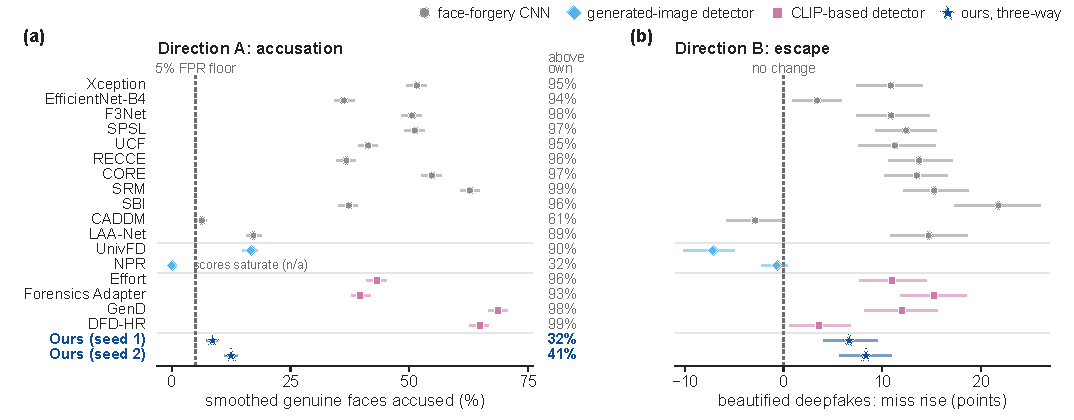
\includegraphics[width=0.98\textwidth]{fig_dirs_v9}
\caption{The two directions on seventeen published detectors and ours, one row per detector. (a) Direction A: share of the
2,210 Smoothing-90 renders accused at the threshold that accuses 5\% of the untouched originals (dot, 95\% interval over pairs;
dashed line: the 5\% floor); the grey number is the threshold-free reading, the share of pairs in which the render scores above
its own original. NPR is n/a because its scores saturate. (b) Direction B: rise of the miss rate on Celeb-DF-B deepfakes from
the app presets alone, re-encoding subtracted (95\% video-cluster intervals). Families from top to bottom: face-forgery CNNs,
generated-image detectors, CLIP-based detectors, ours (two seeds).}
% figs/fig_dirs_v9.pdf, make_fig_dirs_v9.py (= panels b, c of the former fig_teaser_v8b) from alipair_zeroshot_20260929/
% main_claim_A.json (fa_s90_at_5pct, fa_ci, paired_up) and celebdfb_v2_20260927/fair_cdfb.json (d_miss_beauty_only, ci).
\label{fig:dirs}
\end{figure*}

\begin{table}[t]
\centering
\caption{Direction B on Celeb-DF-B. AUC on untreated frames and on frames beautified by the app presets (frame level), FA on
beautified genuine frames, and the rise in the miss rate under beautification minus the rise under re-encoding alone, at the
5\%-FPR threshold of untreated genuine frames. Brackets: 95\% bootstrap over videos. Bold: highest AUC, lowest FA$_b$ and the $\Delta$MISS closest to zero per column (NPR, at chance, is not ranked).}
\label{tab:dirB}
\scriptsize
\setlength{\tabcolsep}{2.5pt}
\begin{tabular}{@{}l c c c c@{}}
\toprule
Detector & AUC untr. & AUC beautified [CI] & FA$_b$ & $\Delta$MISS beauty only [CI] \\
\midrule
% All cells: results/research/celebdfb_v2_20260927/FAIR_cdfb.md (fair_cdfb.py); ours = RU-clipe5 and RU-clipe5-s2 rows.
Xception & 0.811 & 0.737 [0.702, 0.773] & 5.7 & +10.9 [7.4, 14.1] \\
EfficientNet-B4 & 0.811 & 0.762 [0.729, 0.798] & 7.8 & +3.4 [0.9, 5.9] \\
F3Net & 0.798 & 0.731 [0.697, 0.767] & 5.4 & +10.9 [7.4, 14.8] \\
SPSL & 0.781 & 0.727 [0.690, 0.762] & 3.4 & +12.4 [9.3, 15.5] \\
UCF & 0.841 & 0.777 [0.746, 0.808] & 5.7 & +11.3 [7.6, 15.4] \\
RECCE & 0.785 & 0.723 [0.687, 0.758] & 4.1 & +13.8 [10.7, 17.1] \\
CORE & 0.821 & 0.752 [0.718, 0.786] & 4.0 & +13.5 [10.2, 16.6] \\
SRM & 0.789 & 0.733 [0.698, 0.768] & 2.8 & +15.3 [12.1, 18.7] \\
SBI & 0.875 & 0.752 [0.718, 0.785] & \textbf{1.8} & +21.8 [17.3, 26.1] \\
CADDM & 0.886 & 0.762 [0.730, 0.790] & 13.8 & \textbf{$-$2.9} [$-$5.8, 0.1] \\
LAA-Net & 0.889 & 0.698 [0.660, 0.737] & 6.0 & +14.7 [10.9, 18.7] \\
UnivFD & 0.653 & 0.624 [0.579, 0.663] & 7.6 & $-$7.2 [$-$10.2, $-$4.9] \\
NPR & 0.503 & 0.498 [0.453, 0.543] & 3.4 & $-$0.7 [$-$2.2, 0.4] \\
Effort & 0.909 & 0.807 [0.778, 0.836] & 5.4 & +11.0 [7.7, 14.5] \\
Forensics Adapter & 0.909 & 0.828 [0.801, 0.856] & 7.9 & +15.2 [11.9, 18.6] \\
GenD & 0.924 & 0.807 [0.776, 0.836] & 9.9 & +12.0 [8.2, 15.6] \\
DFD-HR & 0.938 & 0.838 [0.807, 0.864] & 14.6 & +3.6 [0.6, 6.8] \\
\midrule
\ours{}, seed 1 & 0.938 & 0.866 [0.841, 0.890] & 9.5 & +6.7 [4.0, 9.5] \\
\ours{}, seed 2 & \textbf{0.941} & \textbf{0.883} [0.861, 0.902] & 6.7 & +8.3 [5.6, 11.0] \\
\bottomrule
\end{tabular}
\end{table}

Table~\ref{tab:dirB} reads the same detectors on deepfake videos beautified by a real app. On this source the accusation
is small, 2--15\% of beautified genuine frames against a 5\% floor for most detectors, and the escape is not.
% FAIR_cdfb.md FA beautified genuine column (SBI 1.8 .. DFD-HR 14.6)
Once the rise under re-encoding is subtracted, fourteen of the seventeen detectors miss 3--22 points
more of the beautified forgeries, with the interval above zero.
% FAIR_cdfb.md last column: 14 detectors with CI > 0 (EfficientNet-B4 +3.4 .. SBI +21.8); UnivFD, NPR, CADDM not
The largest rises belong to SBI, SRM and Forensics Adapter. Every detector that detects the untreated forgeries loses
0.04--0.17 of frame AUC beyond re-encoding (LAA-Net 0.870 to 0.698, SBI 0.861 to 0.752).
% tables/tab_v6b_twosided_main.tex AUC_c - AUC_b column (0.035 SRM .. 0.172 LAA-Net for detectors other than UnivFD/NPR)
Libourel et al.~\cite{libourel2024} reported the AUC drop for three of these detectors; the one-rule reading adds that the
drop is almost entirely misses.

\textbf{Finding 2.} \emph{The same detectors that accuse a smoothed genuine photograph let an app-beautified deepfake video
through: beautification moves forgeries toward the genuine side by 3--22 points for fourteen detectors, and the loss is paid
in misses rather than false alarms.} The two directions appear on different sources because the operating point differs; Finding~5 shows that they are one shift seen from either side of the threshold. For the uploader of Sec.~\ref{sec:intro} this is a 17--69\% chance of accusation at the strongest smoothing level, and for a remote identity check a 3--22 point higher chance that a beautified swap passes; both axes for every detector are in Fig.~\ref{fig:twoaxes}.

\subsection{The cause: training exposure}
\label{sec:exposure}
\begin{figure}[t]
\centering
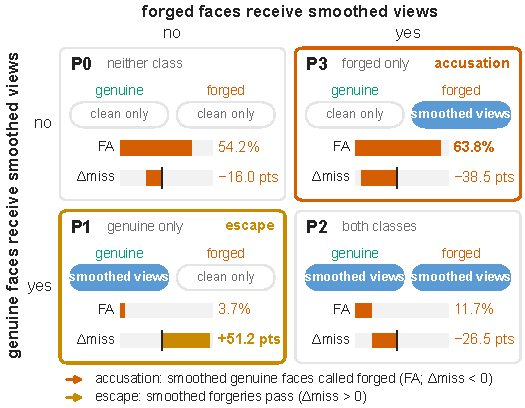
\includegraphics[width=\columnwidth]{fig_exposure_v10}
\caption{The class that receives smoothed training views sets the direction of the error. Four FF++-only arms with the
same architecture, data and recipe, first seed. FA: Smoothing-90 renders accused at the threshold that accuses 5\% of their
originals. $\Delta$miss: change of the miss rate on Celeb-DF-v2 forgeries under strong whole-crop smoothing at the same rule;
a negative change (dark orange) means the arm accuses every smoothed face, a positive one (amber) that smoothed forgeries pass. P1
opens an evasion route; P3 accuses.}
% figs/fig_exposure_v8b.pdf (make_fig_exposure_v8b.py) reads FA = [arm].smoothing90_at_5fpr[0] and dMISS = [arm].miss_rise[2][0]
% (bil21) from results/research/retouch_unified_20260929/p3_readout40.json (same cells as tables/tab_v6_p3.tex and
% tab_v6b_tradeoff_main.tex; cross-checked against smooth_evasion2.json in the script).
\label{fig:exposure}
\end{figure}

\begin{table}[t]
\centering
\caption{The $2\times2$ exposure design. FF++-only CLIP ViT-L/14 LoRA arms, forgery head only, identical except for which
class receives beautified training views (face-local skin smoothing among other edits). Smoothing-90: renders accused at the
5\%-FPR threshold of their originals [95\% over originals]. $\Delta$MISS: change of the miss rate on strongly
whole-crop-smoothed Celeb-DF-v2 forgeries. CDF-B: beautification-only miss rise, three seeds. CDFv2: untreated video AUC. P3
has one seed.}
\label{tab:exposure}
\scriptsize
\setlength{\tabcolsep}{3pt}
\begin{adjustbox}{max width=\columnwidth}
\begin{tabular}{@{}l l c c c c@{}}
\toprule
Arm & smoothed views to & Smoothing-90 [CI] & $\Delta$MISS & CDF-B $\Delta$MISS, 3 seeds & CDFv2 \\
\midrule
% Smoothing-90 and dMISS: tables/tab_v6_p3.tex and tab_v6b_tradeoff_main.tex (FINDINGS.md Addendum 40 table).
% Celeb-DF-B three seeds: tables/tab_exposure.tex (FINDINGS.md 2026-10-11 third seed entry). CDFv2 video: tab_v6b_tradeoff_main.
P0 & neither class & 54.2 [50.5, 58.3] & $-$16.0 & +17.0 / +14.2 / +10.8 & 0.938 \\
P1 & genuine only & 3.7 [2.9, 4.4] & +51.2 & +21.5 / +21.8 / +20.4 & 0.900 \\
P2 & both classes & 11.7 [9.7, 14.3] & $-$26.5 & +9.8 / +10.3 / +12.8 & 0.917 \\
P3 & forged only & 63.8 [59.0, 67.8] & $-$38.5 & -- & 0.943 \\
\bottomrule
\end{tabular}
\end{adjustbox}
\end{table}

To find where the cue comes from we hold architecture, data and recipe fixed and vary only which class receives beautified
views during training (Fig.~\ref{fig:exposure}, Table~\ref{tab:exposure}). The arm without beautified views, P0, already
accuses 54\% of the Smoothing-90 renders, so an FF++-trained detector reads smoothing as forgery evidence out of the box.
Giving the views to genuine faces only (P1) removes the accusation and opens an evasion route. On Celeb-DF-B its
beautification-only miss rise exceeds P0's by 4.5--9.5 points in every one of three seeds (Holm-adjusted $p\le0.01$).
% supplement_v7.tex Sec. S-exposure: P1-P0 +4.5 / +7.5 / +9.5, adjusted p = 0.009
On frames it has never seen it misses 96--100\% of bilaterally smoothed forgeries when smoothing is the only view
(a miss rise of 56--63 points on three seeds).
% FINDINGS.md 2026-10-13 Addendum 33 closed: P1 smoothing only, +56 / +59 / +59 (light), +56 / +60 / +63 (strong)
Giving the views to forged faces only (P3) mirrors P1: it accuses 63.8\% of the renders, 98--100\% of smoothed genuine
frames, and catches smoothed forgeries more often than untreated ones.
% FINDINGS.md rounding note 2026-10-17: P3 63.756 [59.050, 67.784] -> 63.8 [59.0, 67.8]; face-local 98.1 / 100; miss change -25.1 (CDFv2 filters)
Views on both classes (P2) sit in between, and on Celeb-DF-B the P2 minus P0 difference changes sign across seeds, so
symmetric exposure is on average better than none but not reliably so (Table~\ref{S-tab:exposure}).

Two further arms show that smoothing is the operative view. Removing smoothing from the both-class views while keeping colour
grades, filters, whitening and geometric edits brings the accusation back to 55--67\%
% FINDINGS.md Addendum 31: P2 without smoothing 55.3 / 67.2 %
(exposure to smoothing is necessary), and smoothing as the only view on both classes lowers it to 2--5\%
% FINDINGS.md Addendum 32: smoothing-only views both classes 2.3 / 5.3 %
(it is sufficient). The arms do not make the classes more separable; P3's untreated Celeb-DF-v2 video AUC is 0.943 against
0.938 for P0, and exposure moves errors between misses and false alarms.
% tables/tab_v6b_tradeoff_main.tex CDFv2 video column

\textbf{Finding 3.} \emph{The class that receives smoothed views during training sets the sign of the error, and exposure
to smoothing is both necessary and sufficient to set it: genuine-only views teach ``smoothed means genuine'' and open an
evasion route, forged-only views teach the opposite, and no other beautified view substitutes.} This is shortcut
learning~\cite{geirhos2020} under class-dependent augmentation~\cite{balestriero2022}, which Ricker et
al.~\cite{ricker2026biasid} saw for JPEG in two of the four cells; here all four are measured on face forgery, three of
them with replication. In practice this is a warning: a ``filter-robust genuine class'', the recipe a defender would
reach for first, is the P1 cell.

\subsection{The cue: a face smoother than its context}
\label{sec:signature}
% fig_bandenergy_v8b in the supplement (Fig. S-fig:bandenergy); edge-treatment ablation in Sec. S-sec:supp_context

If the detectors reacted to lost texture, the forms that remove more high-frequency energy would be accused more. They are
not (supplement, Fig.~\ref{S-fig:bandenergy}): across seven scripted forms and seventeen detectors the false-alarm rate does not follow the
energy removed above 0.25 cycles per pixel (pooled Spearman $+0.06$);
% FINDINGS.md 2026-10-18 band-energy entry (bandenergy_20261018/BANDENERGY.md): pooled Spearman +0.06
the Gaussian blend removes the most energy and is accused least, the face-local filter removes less and is accused by
nearly every detector. Three contrasts show what the detectors do follow. With the same kernel, confining the smoothing to
the face raises the accusation by 28 points (16 of 17 detectors, $p=5\times10^{-4}$). At equal energy loss an
edge-preserving filter is accused 67 points more than a uniform blur (16 of 17). Only the band 0.02--0.12 cycles per
pixel, the skin relief that a bilateral filter flattens and a Gaussian blend leaves, correlates with the accusation
($\rho=+0.45$).
% BANDENERGY.md via FINDINGS.md 2026-10-18: (i) +28 points 16/17 p = 5e-4; (ii) +67 points 16/17; (iii) rho +0.45

A pre-registered edge ablation locates the cue (Sec.~\ref{S-sec:supp_context}). At the same strength, smoothing only a band
at the face edge is accused at a median of 12\% (7--51\%) by the thirteen face detectors other than CADDM (94\%) and LAA-Net
(65\%), which are trained on blending boundaries, against 92--100\% for the whole face. Smoothing face and surroundings
alike is accused much less (UCF 13.6\%, Effort 30.3\%).
% results/research/retouch_unified_20260929/BDRY38.md (Addendum 57): ring column, fe01 column, whole column
Nor do the texture-poor FF++ families teach it: an FF++-only arm trained without Deepfakes and NeuralTextures accuses
face-local smoothing at 95.5 and 100\% (P0: 95.8 and 100\%; Sec.~\ref{S-sec:noDFNT}), and UnivFD, which never saw FF++, accuses
it too.
% bandenergy_20261018/FFPP_BAND.md; FINDINGS.md 2026-10-23 Addendum 49 (clipe5fbp0F2: fl06 95.5, fl12 100, untreated AUC 0.857)

\textbf{Finding 4.} \emph{The shared cue is a face that is smoother than its own context: skin flattened with kept edges
inside the face while the surroundings keep their texture. It is not blur, not texture loss as such and not the boundary
line.} This is the face-versus-context inconsistency that face-swap detectors are built to find, which face-local
beautification reproduces by construction. It is why Gaussian blur or JPEG as a training view does not remove the accusation (Finding~6; P0 itself trains with blur and JPEG, Sec.~\ref{S-sec:chain}) and why a training-time fix has to use the smoothing signature itself.

\subsection{A threshold cannot separate}
\label{sec:threshold}
\begin{table}[t]
\centering
\caption{A smoothing-conditional threshold. Fixed: fake iff $s>t_0$ with $t_0$ at 5\% FPR on untreated genuine frames.
Conditional: $t_0+\Delta(b)$ with $\Delta$ learnt on FF++ validation genuine renders only, $b$ the smoothing-presence score of
our three-way model. FA on face-local smoothed genuine frames (strength 0.12) and MISS on the same smoothing applied to
forgeries, fixed $\to$ conditional. AUC: both classes smoothed, same form. Recal.\ MISS: miss rate when the threshold is
re-set at 5\% FPR on the smoothed genuine frames themselves (an oracle). Celeb-DF-v2 frames with landmarks.}
\label{tab:bct}
\scriptsize
\setlength{\tabcolsep}{3pt}
\begin{tabular}{@{}l cc cc c c@{}}
\toprule
 & \multicolumn{2}{c}{FA (\%)} & \multicolumn{2}{c}{MISS (\%)} & AUC & Recal. \\
\cmidrule(lr){2-3}\cmidrule(lr){4-5}
Detector & fixed & cond. & fixed & cond. & both sm. & MISS \\
\midrule
% FA / MISS fixed -> BCT: results/research/retouch_unified_20260929/BCT.md (fl12 columns).
% AUC both smoothed and recalibrated miss: RECAL_MISS.md, fl12 column.
Xception & 99.3 & 92.4 & 0.2 & 4.2 & 0.580 & 90.7 \\
SBI & 100.0 & 0.0 & 0.0 & 100.0 & 0.577 & 93.4 \\
CADDM & 99.9 & 0.0 & 0.0 & 100.0 & 0.572 & 91.7 \\
Effort & 99.9 & 0.0 & 0.0 & 100.0 & 0.658 & 84.0 \\
Forensics Adapter & 100.0 & 0.0 & 0.0 & 100.0 & 0.649 & 87.6 \\
GenD & 100.0 & 11.7 & 0.0 & 78.3 & 0.632 & 90.8 \\
DFD-HR & 100.0 & 0.6 & 0.0 & 99.3 & 0.601 & 93.5 \\
\ours{}, forgery head only & 84.5 & 0.1 & 2.5 & 100.0 & 0.755 & 73.7 \\
\bottomrule
\end{tabular}
\end{table}

A fixed threshold accuses smoothed genuine faces (Finding~1). The natural repair is to raise the threshold when smoothing is
detected. We fit such a rule with the smoothing-presence output of our three-way model as the covariate and the shift learnt
on FF++ validation genuine renders only, never on test data (Table~\ref{tab:bct}; every detector in Table~\ref{S-tab:bct}). It works on the genuine side: the
accusation of strongly smoothed genuine faces falls to 0--1\% for Effort, Forensics Adapter, DFD-HR, CADDM and our forgery
head.
% BCT.md fl12 FA: effort 99.9 -> 0.0, fadapter 100 -> 0.0, dfdhr 100 -> 0.6, caddm 99.9 -> 0.0, clipe5b 84.5 -> 0.1
It fails on the forged side at the same moment: 78--100\% of the smoothed forgeries now pass.
% BCT.md fl12 miss: gend 0 -> 78.3, dfdhr 0 -> 99.3, effort / fadapter / caddm / sbi / ours 0 -> 100
The reason is in the sixth column: with both classes smoothed, the AUC between smoothed genuine and smoothed forged faces is
0.60--0.66 for the four CLIP detectors and 0.57--0.58 for SBI and CADDM, so the two score distributions overlap and any
threshold that clears one clears the other.
% RECAL_MISS.md fl12: effort 0.658, fadapter 0.649, gend 0.632, dfdhr 0.601, sbi 0.577, caddm 0.572
Even an oracle that re-sets the threshold on the smoothed genuine frames themselves leaves every published detector
missing 67--100\% of the smoothed forgeries at the two strong forms, and ours 52--77\% (Table~\ref{S-tab:recal}).
% RECAL_MISS.md: published bil15 67.7-100, fl12 84.0-100; ours (ref, lam0, SIC) 52.0-76.7

\textbf{Finding 5.} \emph{No threshold rule separates smoothed genuine from smoothed forged faces for any of the
detectors: under skin smoothing the two score distributions coincide, so the accusation and the escape are one distribution
read from two sides, and a decision rule can only move the error from one side to the other.} Calibration on untreated data,
the remedy proposed for smartphone photographs~\cite{laionmobile2026}, does not apply here, because the problem is not where
the threshold sits but that there is no threshold to find.

\subsection{Training only trades}
\label{sec:sic}
\begin{table*}[t]
\centering
\caption{Smoothing-invariant consistency (SIC) against the same model trained without it (forgery head only, same data,
views, seeds and checkpoint rule). FA: smoothed genuine Celeb-DF-v2 frames called fake at the 5\%-FPR rule (face-local 0.06 /
0.12, whole-crop bilateral 15); S-90: commercial Smoothing-90 renders accused; $\Delta$miss: miss rise on face-local 0.12
smoothed forgeries; untreated video AUC on Celeb-DF-v2 and DFD; Celeb-DF-B AUC under the presets; DF40 reenactment video AUC
(FF++ domain); bars passed of six pre-registered bars. The view-only control ($\lambda=0$) draws the same smoothed copy for
both classes without the penalty.}
\label{tab:sic}
\footnotesize
\begin{adjustbox}{max width=\textwidth}\begin{tabular}{@{}lcccccccccccc@{}}
\toprule
Model & seed & \multicolumn{3}{c}{smoothed genuine accused (\%)} & S-90 & $\Delta$miss & \multicolumn{2}{c}{untreated video AUC} & Celeb-DF-B & DF40 FR & bars \\
 & & fl 0.06 & fl 0.12 & bil 15 & acc.\ \% & fl 0.12 & CDFv2 & DFD & AUC & ff & passed \\
\midrule
forgery head only, no rule & 1 & 51.6 & 84.5 & 35.5 & 9.1 & $-$34.0 & 0.956 & 0.987 & 0.866 & 0.842 & -- \\
\midrule
symmetric view only ($\lambda=0$) & 1 & 53.9 & 91.8 & 1.6 & 11.9 & $-$40.1 & 0.943 & 0.975 & 0.891 & 0.835 & 3/6 \\
SIC, $\lambda=0.03$ & 1 & 5.0 & 3.3 & 9.6 & 11.2 & 24.4 & 0.946 & 0.979 & 0.886 & 0.750 & 4/6 \\
SIC, $\lambda=0.03$ & 2 & 3.8 & 3.5 & 8.8 & 15.0 & 20.4 & 0.933 & 0.975 & 0.876 & 0.777 & 2/6 \\
SIC, $\lambda=0.1$ & 1 & 6.5 & 4.2 & 9.9 & 10.5 & 15.8 & 0.930 & 0.980 & 0.871 & 0.774 & 3/6 \\
SIC, $\lambda=0.1$ & 2 & 4.6 & 4.6 & 8.5 & 8.1 & 17.6 & 0.929 & 0.974 & 0.868 & 0.771 & 2/6 \\
SIC, $\lambda=0.3$ & 1 & 6.0 & 4.2 & 8.1 & 12.8 & 9.5 & 0.898 & 0.971 & 0.840 & 0.692 & 2/6 \\
SIC, $\lambda=1$ & 1 & 5.8 & 4.4 & 5.8 & 2.1 & 9.7 & 0.907 & 0.986 & 0.835 & 0.768 & 2/6 \\
SIC, $\lambda=1$ & 2 & 6.2 & 5.5 & 6.3 & 12.3 & 6.1 & 0.844 & 0.968 & 0.804 & 0.746 & 2/6 \\
one-sided penalty & 1 & 0.1 & 0.1 & 0.0 & 9.2 & 56.5 & 0.954 & 0.980 & 0.880 & 0.794 & 4/6 \\
one-sided penalty & 2 & 0.1 & 0.0 & 0.0 & 10.4 & 47.3 & 0.929 & 0.975 & 0.860 & 0.775 & 2/6 \\
Gaussian view (ablation) & 1 & 5.8 & 19.5 & 1.1 & 3.5 & $-$13.5 & 0.855 & 0.971 & 0.819 & 0.782 & 1/6 \\
Gaussian view (ablation) & 2 & 5.9 & 14.5 & 1.3 & 8.7 & $-$9.3 & 0.848 & 0.960 & 0.821 & 0.784 & 2/6 \\
SIC, $\lambda=1$, FF++ only & 1 & 7.4 & 6.8 & 5.3 & 7.0 & 4.8 & 0.856 & 0.979 & 0.829 & 0.674 & 2/6 \\
\bottomrule
\end{tabular}
\end{adjustbox}
% tables/tab_sic.tex is generated by make_tab_sic.py from results/research/retouch_unified_20260929/readout46.json (READOUT46.md).
\end{table*}
% fig_sic_curve_v8b moved to the supplement (Fig. S-fig:siccurve) on 2026-10-22 to make room for fig_method_v8b

If the cue is set in training, can training remove it? We tested the rule that Finding~3 and Finding~4 suggest: one
skin-smoothing operator drawn identically for every training item of every class, and a penalty $\lambda$ on the change of
the forgery logit between the clean item and its smoothed copy, with the clean logit held as a stop-gradient target. Bars
were written before training (Table~\ref{S-tab:sicbars}). Table~\ref{tab:sic} gives the family and Fig.~\ref{S-fig:siccurve} in the supplement plots it. Every penalty
weight from 0.03 upward removes the face-local accusation (3--7\% on smoothed genuine frames, against 52 and 85\% for the
reference), and the symmetric view alone ($\lambda=0$) does not (54 and 92\% at the two face-local strengths), so the
penalty does the work. The commercial renders do not separate the arms: the reference already accuses only 9.1\% of them
and the penalty arms 2--13\%.

% READOUT46.md: lam0 fl06 53.9 / fl12 91.8; SIC arms fl 3.3-7.4, S-90 2.1-12.8
% 2026-10-23: reference S-90 corrected from a hand-typed 40.6 to 9.1 (readout46.ali("clipe5b_s20260929"); CONSISTENCY_AUDIT_20261023 #1)

The cost has two faces that trade against each other along $\lambda$. At large weights the clean forgery score is pulled
toward its smoothed copy and untreated detection falls (Celeb-DF-v2 video AUC 0.907 at $\lambda=1$ against 0.956 without
the rule); at small weights detection is kept (0.946 at $\lambda=0.03$) but the smoothed forgery's score falls with the
genuine one and its miss rises by 24 points. A one-sided penalty that forbids only a rise of the logit is the limit of that
direction: untreated AUC 0.954 and 56 points more smoothed forgeries missed. A Gaussian blur of the same support in place of
the smoothing operator fails the accusation bar at the strong face-local form (19.5\%) and opens the bilateral evasion. DF40
reenactment is 0.06--0.09 below the reference at every weight, the one bar no member passes.
% READOUT46.md / FINDINGS.md 2026-10-19 20:30 family table: sg l1 0.907, l0.03 0.946 (+24), hinge 0.954 (+56), Gaussian fl12 19.5, DF40 -0.06..-0.09

The penalty buys the operating point and leaves separability where the view put it. The deciding control is the $\lambda=0$ model read with
the oracle smoothing-conditional threshold of Finding~5. With both classes smoothed it keeps an AUC of 0.832 (bilateral) and
0.764 (face-local), against 0.790 and 0.778 for SIC at $\lambda=1$ and 0.802 and 0.778 at $\lambda=0.1$. Its
recalibrated miss rate (57 and 77\%) is not higher than SIC's (64--73\% on two seeds).
% RECAL_MISS.md: lam0 0.832 / 57.4 (bil15), 0.764 / 76.7 (fl12); SIC-sg s1 0.790 / 64.5, 0.778 / 64.0; s2 0.733 / 73.0, 0.720 / 72.8
% READOUT46.md both-smoothed AUC: lam0 0.8318 / 0.7639; sg 0.7897 / 0.7782; sgl01 0.8019 / 0.7783
SIC therefore amounts to a symmetric view plus one threshold shift that carries across untreated and smoothed
inputs; it does not keep separation that the view alone would lose.

Nor does a routed expert. A second model trained only on
smoothed copies, selected by the smoothing score, clears the accusation (face-local 51--52 and 80--85\% to 1--2\%) and raises
the miss on smoothed forgeries by 41--46 points; its both-classes-smoothed AUC is below the untreated detector's on seven
of the eight forms, on both seeds (Table~\ref{S-tab:sce}).
% results/research/retouch_unified_20260929/SCE_s1.md and SCE_s2.md: fl06 51.6/51.2 -> 0.9/2.1, fl12 84.5/79.9 -> 1.3/1.3;
% miss rise 41.7/44.4 (s1), 40.6/46.0 (s2); B below A on 7 of 8 forms on both seeds (fl12 the exception)
Nor does a rule at test time. Calling a face forged only if it also exceeds the threshold after its whole crop is smoothed,
which removes the face-versus-context contrast, clears the accusation for 10 of 15 face detectors. At a matched false-alarm
rate on the smoothed genuine frames, however, it misses smoothed forgeries within a few points of the recalibrated single
score for all fifteen (Sec.~\ref{S-sec:supp_context}).
% results/research/retouch_unified_20260929/CTX38.md (Addendum 61): prediction 1 10/15, prediction 2 0/15, KILLED

The loss is not confined to the shortcut arms: with both classes smoothed, every one of the seventeen published detectors
loses AUC, by 0.06--0.28 at
the strong face-local form for the sixteen that are above chance, and the $\lambda=0$ model, which saw smoothed views of both
classes in training, still loses 0.061 and 0.129.
% RECAL_MISS.md untreated vs fl12 (published other than NPR: 0.060 F3Net .. 0.281 LAA-Net); lam0 0.893 -> 0.832 / 0.764
Part of the forgery evidence is erased by smoothing itself, beyond the shortcut; how much of the published detectors'
loss comes from the shortcut being pushed to its ceiling and how much from erased evidence cannot be separated with these
data, and we call the $\lambda=0$ loss a measured loss, not a bound.

\textbf{Finding 6.} \emph{Training can move the error but not remove it. A class-symmetric smoothing view with a
consistency penalty takes the accusation of smoothed genuine faces from 85\% to 4\% at a cost in untreated detection, but it is
a smoothing-conditional recalibration, since the view-only model read with a conditional threshold separates smoothed
faces at least as well. A routed expert and test-time context matching are recalibrations too, and with both classes
smoothed every detector, published or ours, loses separability.}
% 85 -> 4: tab_sic.tex, reference fl12 84.5 vs SIC lambda 0.1 fl12 4.2
A fix for the accusation has to be bought with misses on smoothed forgeries or with untreated detection, and a
paper that reports only one of the three is reporting a point on this curve, not a solution.

\subsection{Identity: the channel that survives}
\label{sec:identity}
Smoothing erases texture evidence but not who the person is. We score the ArcFace distance between each Celeb-DF-B frame and
a reference of the claimed person, made from up to four of that person's Celeb-DF-v2 genuine videos outside the benchmark, with
four predictions written before any frame was embedded (Table~\ref{S-tab:cdfbid}; scripted forms and ICT-Ref~\cite{ict2022} in
Tables~\ref{S-tab:idref} and~\ref{S-tab:ict}). Its video AUC is 1.000 untreated, beautified and re-encoded. Re-thresholded to
accuse 5\% of the beautified genuine frames, it misses 0.6\% of the beautified forgeries, against 46--72\% for the texture
detectors (ours 51.1 and 46.2\%, Effort 51.9\%, SBI 69.6\%, CADDM 72.1\%). Its operating point still moves: at the untreated
threshold its false alarm on beautified genuine frames rises by 8.5 points [6.4, 10.6] beyond re-encoding, short of the
predicted 10. A rank-mean fusion with a texture detector meets the pre-declared bars with our model (false-alarm rise +7.7, miss
rise +2.9) but not with Effort (miss rise +8.5 [5.4, 11.5] against a bar of 5), so no fusion method is claimed. Two of the four predictions hold (the stable AUC and the recalibrated miss) and two do not (the fusion bars and the size of the operating-point shift).
% results/research/retouch_unified_20260929/CDFB_ID.md (Addendum 62): identity vAUC 1.000/1.000/1.000; dFA +8.5 [+6.4, +10.6];
% last column; fusion_ours+identity, fusion_effort+identity rows. Scripted forms: ID_REF.md; ICT-Ref: ICT_PROBE.md

\textbf{Finding 7.} \emph{A recognition embedding compared with a reference of the claimed person is the one channel we tested that beautification leaves: under real app presets on face swaps its separation does not move while every texture detector loses most of its own. Its operating point does move, so a detector that uses it needs a beautification-aware threshold.} The channel
needs a reference, without which it is near chance (AUC 0.59); it is blind to reenactment and attribute edits, which keep the
identity; and Celeb-DF swaps are easy for it, so the 1.000 is an upper bound. Identity evidence is prior art~\cite{identitydriven2020,idreveal2021,ict2022,yin2026}, including detectors personalised on reference images of a protected identity~\cite{vipguard2025}, and the stable-AUC, moving-threshold pattern under beauty filters is known from face recognition~\cite{mirabet2025}; those works build detectors, whereas the measurement of the channel under beautification is new.
% AUC 0.59 without a reference: FFPP_ARCFACE.md (Addendum 53)
A reference of the claimed person does not, however, catch the beautification itself. Across one person's untreated
videos, the share of score variance that belongs to the person (intraclass correlation, ICC) is 0.14 for our beautified score,
0.12--0.46 for the texture detectors and 0.06--0.32 for skin texture and colour; subtracting the person's reference mean leaves
the preset-only AUC where it was (ours 0.720 and 0.718, gain $-0.002$ [$-0.015$, 0.011]; seven texture detectors $-0.023$ to
$+0.005$). Face width is identity-stable (ICC 0.66): on the benchmark's genuine videos narrowed by 2.25\%, the same reference
lifts the video AUC of a landmark width ratio from 0.635 to 0.727 (gain $+0.092$ [0.067, 0.116], short of the pre-declared
$+0.10$), while our beautified score gains nothing on the same images. The variation that hides a light colour or texture edit
belongs to the capture, not to the person, so a reference helps only for edits of the person's geometry, the part that
differential retouching detection reads from landmarks~\cite{rathgeb2020diff}. A 3D morphable-model fit~\cite{tddfav2} is
steadier across one person's videos but registers 0.2\% of the 2.25\% narrowing, so it is the wrong instrument for edits of
this size.
% results/research/refcond_20261029/REFCOND_65.md (Add. 65): C1 ours 0.720 -> 0.718, gain -0.002 [-0.015, 0.011]; ICC ours 0.14,
% texture detectors 0.12-0.46, skin texture 0.06-0.07, skin colour 0.14-0.32, face width 0.66. GEO68.md (Add. 68): face width,
% jaw 0.10 (-2.25 %), 0.635 -> 0.727, gain +0.092 [+0.067, +0.116]; ours +0.002..+0.010. GEO3D_69.md (Add. 69): -0.22 %, gain +0.028.

\begin{figure}[t]
\centering
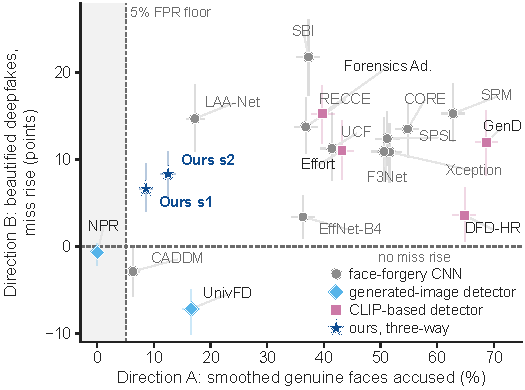
\includegraphics[width=\columnwidth]{fig_twoaxis_v10}
\caption{No published detector is low on both axes; ours and CADDM sit in the lower-left corner. Each point is one detector: Direction A, Smoothing-90 renders accused at the threshold that
accuses 5\% of the originals (Table~\ref{tab:dirA}), against Direction B, the beautification-only miss rise on Celeb-DF-B
(Table~\ref{tab:dirB}); bars are the 95\% intervals, NPR is saturated at zero, EffNet-B4 is EfficientNet-B4. The lower-left corner holds our two seeds and CADDM, whose interval contains zero but which accuses 13.8\% of beautified
genuine frames.}
% figs/fig_twoaxis_v10.pdf (make_fig_twoaxis_v10.py; = v8b with one marker size and stronger label repulsion) from alipair_zeroshot_20260929/main_claim_A.json (fa_s90_at_5pct, fa_ci)
% and celebdfb_v2_20260927/fair_cdfb.json (d_miss_beauty_only, ci, auc_untreated).
\label{fig:twoaxes}
\end{figure}

% ----------------------------------------------------------------------------
\section{A Companion Three-Way Detector}
\label{sec:companion}
Our companion model (Fig.~\ref{fig:method}b) is the detector that Findings~3 and~6 call for: smoothing on both classes in training, and the forgery decision read from a head that is not asked to be smoothing-invariant. Its beautified attribute is optional, since on the same data a forgery-head-only model is at least as good on every forgery number and better on reenactment, and the model was trained on more data than the published detectors, so the comparisons below are an audit reference, not a ranking.

\textbf{System and training recipe.} The backbone is a frozen CLIP ViT-L/14~\cite{clip} with rank-16 LoRA~\cite{lora} on the
query, key, value and output projections of all 24 blocks (3.2\,M of 306\,M parameters trained). Two linear heads on the CLS
token give the forged logit $z_f$ and the beautified logit $z_b$; with $f=\sigma(z_f)$ and $b=\sigma(z_b)$ the three classes
are fake $f$, beautified $(1-f)b$ and real $(1-f)(1-b)$, and the decision reads $P(\text{fake})=f$ only. An operation head
(presence and amount of four operations) and a linear layer on the 256 patch tokens, which gives a $16\times16$ evidence map
trained against the exact footprint of each edit, are trained alongside and are not read by the decision (supplement).
% results/research/retouch_unified_20260929/train_ru5.py (RUCLIP5: fz, pres, q, ev) and train_ru_clip.py (LoRALinear r=16 on
% q_proj/k_proj/v_proj/out_proj of every encoder layer); 3.2 M = "trainable 3.16 M" in train_ru_clipe5_s20260929.log
Each training step builds a genuine, a beautified and a forged item from one genuine FF++ c23~\cite{ffpp} or FFHQ frame
(Fig.~\ref{fig:method}b; sources in the supplement), the forged item beautified with probability 0.5 so that both classes
receive the views; the beautified renders come from two retouching services that are sister services of the test service.
% manifest_train.tsv / manifest_val.tsv src counts (ffpp_real 41,512; ffhq_orig 7,015 + 816; ffpp_fake 41,526; tencent 6,924 +
% megvii 11,810; ffpp_filter 41,512); train_ru_clipe5_s20260929.log "single 50,112 | parts 61,510"; recipe: train_ru5.py
% RUData5.__getitem__ (self-blend and observed forgeries beautified on top with p = 0.5)
The test service itself is never seen. Training: 224\,px, AdamW at $10^{-4}$, 8 epochs; checkpoints are chosen on validation
data only, by a balanced criterion that penalises originals sent to the beautified class (supplement).


\textbf{Both axes.} On the retouching pairs the model ranks the render above its original in 32.5 and 41.3\% of pairs on
its two seeds and accuses 8.6 and 12.5\% (Table~\ref{tab:dirA}); its native decision sends 98.8 and 99.2\% of the renders to
beautified. On Celeb-DF-B it keeps the highest AUC under the presets, 0.866 and 0.883, and its beautification-only miss rise
of 6.7 and 8.3 points is smaller than that of Forensics Adapter, SBI and GenD but larger than that of DFD-HR and CADDM
(Table~\ref{tab:dirB}). CADDM is lower on both raw axes (6.3\% and $-2.9$ points) at a beautified AUC of 0.762
(Fig.~\ref{fig:twoaxes}).
% MAIN_CLAIMS_20261022.md Direction A and B, ours s1 / s2 rows and paired-difference lines

The controlled comparison is the same architecture with and without
beautified views (Table~\ref{tab:exposure}). Both-class views take the accusation from 54.2 to 11.7\% and change the escape by
$-7.2$, $-4.0$ and $+2.0$ points over three seeds. On the full data a forgery-head-only model is as good on both axes
within seed spread (9.1 and 6.5\% accused, beautified AUC 0.896 and 0.904), so the gain comes from the training data, not
from the third class.
% tab_exposure.tex (P2 - P0 per seed); BCT.md clipe5b rows; FAIR_cdfb.md RU-clipe5b rows

\textbf{Untreated detection.} On Celeb-DF-v2 and DFD the model is on par with all four CLIP detectors (frame AUC 0.891 and
0.942, video 0.947; no paired interval excludes zero in either direction; Table~\ref{S-tab:reproduce}).
% tables/tab_v6b_reproduce.tex (former Table VI of v8)
On DF40 face swaps it is at Effort's level in the FF++ domain and
0.03 below it in the Celeb-DF domain (video AUC 0.952 and 0.905 against 0.944 and 0.935; no paired interval was computed).
% tables/tab_v6b_df40_main.tex, FS columns

\textbf{Costs.} Four are measured. On DF40 reenactment the model is behind: 0.718 and 0.502 in the two domains against
0.808 and 0.710 for Effort and 0.935 and 0.828 for GenD, and a forgery-head-only model on the same data is 0.08--0.15 above
it, so the shared beautified head costs reenactment (Table~\ref{S-tab:v4df40full}).
% tables/tab_v6b_df40_main.tex FR columns; tab_v6b_seeds.tex block (B): DF40 FR +0.124 / +0.145 (seed 1)
It sends 20.8 and 19.6\% of the service's untouched originals to the beautified class,
% MAIN_CLAIM_A.md native decision: orig filter 20.8 (s1) / 19.6 (s2)
a cost the retouching source pays for the low accusation. Its beautified class is itself an escape route: on Celeb-DF-B it
sends 16.6 and 16.1\% of the beautified deepfakes to beautified, against 3.6 and 3.9\% of the same deepfakes untreated; these
count as misses in Table~\ref{tab:dirB}.
% FINDINGS.md Addendum 54 last paragraph (three-way decision on Celeb-DF-B)


\textbf{Operation scores.} Its four operation scores are reliable only for smoothing: on the
service's single-operation renders the presence head recovers smoothing in 94\% of cases but eye
enlarging in 20\%, face slimming in 32\% and whitening in 38\%,
% READOUT46.md attribute_main_same_seed presence TP: smooth 0.943, eye 0.196, jaw 0.322, white 0.375
and on real-app filters almost none (recall 0.003--0.24; Table~\ref{S-tab:fbops}).
% FB_OPS.md clipe5_s20260929, all: eye 0.003, jaw 0.032, white 0.176, smooth 0.243
The operation names describe the training family rather than beautification in general, and we no longer claim them.

% ----------------------------------------------------------------------------
\section{Limitations and What We No Longer Claim}
\label{sec:limits}
The measurement covers one commercial retouching service, four app presets on one video dataset, seven scripted smoothing
forms and one open-source beauty engine. The retouching source was read during the study and is an analysis set. GPUPixel's
skin smoothing, a source no design decision touched, reproduces the accusation (14 of 15 face detectors above
15\% at its strongest level, against 2.4--4.9\% for the same pipeline without smoothing) but not the ranking of the detectors (Spearman
0.24 against the scripted bilateral form). It is a port of the shader, not the compiled library.
% results/research/retouch_unified_20260929/GPX38.md (Addendum 54)
 Celeb-DF-B shares its genuine videos
and identities with Celeb-DF-v2, on which every detector in the table was evaluated by its authors, so it is not identity
disjoint. P3 and several SIC arms have one seed, and no non-CLIP pipeline was trained with the rule. Effort and DFD-HR were
not reproduced at their published Celeb-DF-v2 numbers (Table~\ref{S-tab:reproduce}), and we compare against their released
weights.

Four claims of earlier drafts are withdrawn and one result is moved out. The FF++ texture origin of the cue: an arm trained
without Deepfakes and NeuralTextures accuses as much (Sec.~\ref{sec:signature}). Instagram AR filters: the renders cannot be separated from the OpenFilter
capture pipeline (Sec.~\ref{sec:protocol}) and our models accuse them as much as the CLIP detectors (Table~\ref{S-tab:ar}).
% tables/tab_v6b_ar.tex FairBeauty accused: oursF 75.1, oursB 79.0 / 82.1; Effort 67.8, FA 63.9, GenD 75.6, DFD-HR 85.9
% FINDINGS.md 2026-10-22 16:40 Addendum 56: clipe5M 78.1 vs clipe5 75.1
Operation naming: the four operation scores identify smoothing on the training family and little else
(Sec.~\ref{sec:companion}). Language-model explanations did not differ from template sentences in any measured respect and
were removed; localisation of part-level forgeries and its restoration test are in the supplement.
Two further channels were tested without training and closed: weighting the texture--identity fusion by the model's own
beautified estimate moves the error from misses to false alarms, since the estimate rises on beautified genuine faces as on
beautified forgeries; and the pulse signal of remote photoplethysmography has no separation to lose on Celeb-DF (video AUC
0.51), because the swaps inherit the driving video's pulse (peak frequency agreement with the source video 44\% against
19\% by chance).
% results/research/retouch_unified_20260929/CDFB_GATE.md (Addendum 63): dFA +11.5..+17.1, dMISS -5.4..-10.4
% results/research/retouch_unified_20260929/CDFB_RPPG.md (Addendum 64): AUC 0.514; peak agreement 0.439 vs 0.187

% ----------------------------------------------------------------------------
\section{Related Work}
\label{sec:related}
Four strands of prior work touch this measurement: beautification evaluations, benign-edit benchmarks, shortcut learning and identity evidence. Libourel et al.~\cite{libourel2024}, Saeed et al.~\cite{saeed2025} and Concas et al.~\cite{concas2025} are discussed in
Sec.~\ref{sec:intro}; Libourel et al.\ close by recommending a dedicated filter-detection stage, which the companion model's
beautified head is. Tariq et al.~\cite{moire2025} benchmark detectors against moir\'e and name beautification as future work; von Stryk and
Keuper~\cite{laionmobile2026} find that false alarms on smartphone photographs follow threshold calibration, which Finding~5
rules out for skin smoothing.

Retouching detection and
restoration~\cite{bharati2016,jain2018,wang2019photoshop,retouchingffhq,frrffusion,mofrr,reface} have no forgery class;
OpenFilter~\cite{openfilter2022} renders AR filters; Liu et al.~\cite{miea2026} attribute editing tools in a closed set;
perturbation benchmarks~\cite{deeperforensics2020,hendrycks2019} treat edits as corruptions of one class.

Shortcut learning~\cite{geirhos2020}, group shifts~\cite{sagawa2020} and class-dependent augmentation~\cite{balestriero2022} describe
the mechanism of Finding~3; Ricker et al.~\cite{ricker2026biasid} found the sign flip for JPEG with two cells. CORE~\cite{core}
ties representations across generic augmentations and still ranks a smoothed genuine face above its original in 97\% of
pairs; the alpha-blending hypothesis~\cite{alphablend2026} holds that frame-based detectors read compositing artefacts; our
edge-treatment ablation shows that face-local skin smoothing produces that inconsistency with no boundary line at all.

Identity-referenced detection~\cite{identitydriven2020,idreveal2021,ict2022,yin2026,vipguard2025} and face recognition under beauty filters~\cite{mirabet2025} are the prior art for Finding~7; DeepfakeBench~\cite{deepfakebench} and
DF40~\cite{df40} provide the checkpoints and test sets.

% ----------------------------------------------------------------------------
\section{Conclusion}
Seventeen published face-forgery detectors read skin smoothing as forgery evidence: one cue accuses the smoothed genuine
photograph and lets the app-beautified deepfake through. The cue is set by which class saw smoothing in training. It is the
contrast between a flattened face and its untouched surroundings, which face-local beautification produces and face-swap
detectors are built to flag. No threshold, routing, consistency loss or test-time rule removes it, because, once both
classes are smoothed, no score separates them.
What beautification does not erase is who the person is: identity against a reference keeps its separation under real app
presets, provided the threshold is set on beautified genuine faces. The manifests, the rule, the paired reader, the per-detector result files and the pre-registration log are released.

\bibliographystyle{IEEEtran}
\bibliography{refs_v8}
\end{document}
